\documentclass[11 pt]{article}

\usepackage{titlesec}
\usepackage[dvipdfmx]{graphicx}
\usepackage{bmpsize}
\usepackage{amsmath,mathrsfs}
\usepackage{amssymb}
\usepackage{enumerate}
\usepackage{grffile}
\usepackage{hyperref}
\hypersetup{
    colorlinks,
    citecolor=black,
    filecolor=black,
    linkcolor=black,
    urlcolor=black
}
\usepackage[margin=1in]{geometry}
\usepackage[font={scriptsize}]{caption}
\title{Lab Notes for Compressed Sensing Coding}


\newcommand{\me}{\mathrm{e}}
\newcommand{\ep}{\varepsilon}
\newcommand{\sectionbreak}{\clearpage\newpage}
\newcommand{\mitem}{\item[--]}
\newcommand{\bo}{\noindent\textbf}
\newcommand{\etal}{\emph{et. al.}}
\newcommand{\matlab}{\textsc{Matlab }}
\let\oldsection\section
\renewcommand\section{\clearpage\newpage\oldsection}

\usepackage[nodisplayskipstretch]{setspace}
\usepackage{fancyhdr}
\pagestyle{fancy}

\fancyhead[R]{Salerno}
\fancyhead[C]{Lab Notes for Compressed Sensing Coding}
\fancyhead[L]{MICe}

\begin{document}

\vfill

  \begin{titlepage}
    \vspace*{\fill}
    \begin{center}
      {\huge {Lab Notes for Compressed Sensing Coding}}\\[0.5cm]
      {\large {Anthony Salerno}}\\[0.4cm]
      \today
    \end{center}
    \vspace*{\fill}
  \end{titlepage}

\clearpage
\newpage

\tableofcontents

\newpage

\section{Proof of Principle (02.17.15 - 02.23.15)}

\bo{Introduction}\\
Beginning work on the ``Proof of Principle" as per the 12.19.14 Meeting Notes - Plan 2

The notes state that we are to:
\begin{itemize}
  \item Pick one slice - extract slice from dataset with FT on RO (i.e. in dim space) and no FT on PE1 and PE2 (aka PE and SL)
  \item Isotropic undersampling (I think this is a bad idea)
  \item Recon slices independently with Lustig code (using $\lambda_2 psi[m] + \lambda_1 TV[m]$)
  \item Add a directional similarity term to the recon (so we can recon similar slices simulataneously) ($\lambda_3 ||m_j - m_k||_2 f(\vec{d_j} \cdot \vec{d_k}))$
  \item However, the form of $f((\vec{d_j}\cdot \vec{d_k}))$ is still unknown
\end{itemize}

\noindent Note that the git repository for this work can be found at \url{https://github.com/aasalerno/Lustig}. For pre-emptive notes on the code that Lustig wrote, please see \verb!demo_SheppLoganTV_Notes.txt!. \\ \\

\subsection{Preamble...}
\subsubsection{Hypothesis}
To begin, today we should be able to get a decent code running that can do Lustig's code on any specified slice that we choose. I expect that the code will work as expected and provide a good rendition of the undersampled data with minimal alterations required. The hope is that we can use the basis of the code as an engine (that will need some optimization) in order to work with the data as we so hope.


    \subsubsection{Notes - Unpolished}
    First spent a ridiculous amount of time getting \LaTeX up and running on this computer... But it works now! 

    The code is written both on my computer as well as on the lab computers -- via a central git on github -- using the same datasets as required. The datasets in use are Jacob's data, reconstructed purely using the standard recon algorithm (that is, no \matlab involved).

    For all pushes and pulls, see the github repository. There are many (and it can be mapped by day!)

    The code is to be written such that it is built and any values that are above 1-sampFac will be included. This means that when we are actually tacking on the $r$ correction, we need to do it as $1-\frac{r}{\text{max}(r)}$

    Seem to have a problem with the values that I'm getting. The outer portions of k-space seem to have almost no chance of being chosen. With a penalty threshold of only 0.25 (given a sampFac of 0.5), only 40\% of values are chosen. Most of the lost points are on the corners of $k$-space, so this may be ok... However, I need to look into \textbf{possibly making the CS type sequence specific, for things like cylindrical acquisition}. \\ \\ 

  \noindent Date: 02/20/15

    As of about 11:00 (commit 6a9cfb111c508df0af9a7222ba277ef118ba147), the code \verb!testMap.m! is up and running. It will be used in order to actually build the map of what we are undersampling and then this will be pumped into an adapted version of Lustig's code in order to get it up and running.

    Encountered a bit of an issue with how the data is obtained. Since this information is only the magnitude of the data, I'm going to make a version that can handle taking the real and imaginary parts of the data, then feeding that through to the next set of functions.

    As of 12:08 PM, functionality has been added for the function to handle two files containing the real and imaginary parts of the $k$-space information!

    Now, we want to add in the CS part of the code. Here is where things become a little painful, but we can look at the datasets and actually do what is done in CS.

    For some unapparent reason, the code doesn't seem to want to work. This is really annoying and irritating as the error seems to be stemming from the raw files, which may render a tonne of previous work that I've done utterly useless. Ok, scratch that -- the issue was my method of plotting. I wasn't plotting the abs of the data. 

    As of about 5:00 it is working. I'm going to git push it and go home. \\ \\

\noindent Date: 02/23/15

    Upon a first look at the doce that I wrote last week (adapted from \verb!demo_SheppLoganTV.m!, the code doesn't seem to have too great of an effect. The differences between the ``im\_dc" (density corrected original) and the CS reconstructed data is on the order of $10^{-9}$, when the data is on the order of 1.

    \begin{itemize}
      \item One of the first things that I should try is to change the TV and L1 penalties as they are currently set to 0.01 each. This may be too low to have an effect on real data -- the code that I am adapting from is using a numerical phantom.
      \item The next step would be to try different slices or different data. Perhaps the noisiness of this data is causing a problem, but can be fixed with some more phase corrections.
    \end{itemize}

    I changed the values of the two penalties ($\lambda_1$ and $\lambda_2$), increasing them by a factor of 10, each becoming 0.1. The overall residual became a little bit larger, but is still on the order of $10^{-9}$, which is negligible.

    In order to make the data make a bit more sense (i.e. make sure I'm not making a stupid mistake on how I'm building the filter, etc) I'm going to use Lustig's method of buiding the undersampling pattern.

    I changed the code \verb!testMap.m! pretty substantially, so see github for a previous version. The alterations were made to try and use the other undersampling pattern. One thing that I may do later is alter Lustig's PDF that is produced by tacking on the directionality afterwards.

    After changing to Lustig's method of undersampling, we see some bigger differences, but, the undersampling kind of makes it look pretty bad. It may be how the FT (using this `\verb!p2DFT!') instead of just doing an FFT as it is done in \matlab. This seems like something weird that they don't need to do, as it just makes the data look bad... Though there must be a reason for this

    As it stands -- 4:00PM 02/23/15 -- this is as far as I can go without further understanding how well everything is going to work for the perpendicular and parallel to the gradient direction for the undersampling technique.

\subsection{Simulations}
    \subsubsection{Preamble}
    Here what we want to ensure is that by applying specific filters, we are obtaining what we expect. The expectation is that using a mask that is parallel to the gradient direction (applied in $k$-space) is going to look significantly worse than a mask applied perpendicular to the gradient direction.

  \subsection{Hypothesis}
  Using a simulation, we will be able to tell distinct differences beteween the use of the two different maps. The map using a perpendicular mask on the undersampled $k$-space will look better than the data undersampled using the parallel mask, as the smearing will not be as bad in the cross direction of the diffusion.

  The code is written in \verb!buildLambda.m!. It is currently built just to handle a 2D case and then \emph{eventually} handled to build a 3D. In order to make it work with the code, an idea is to make it have a $z$-stack (in our case, a $y$ stack, or a `read-out" stack). \\ \\ 

\section{Analysis of CS Code -- Sanity Check (03.10.15)}
\noindent Date: 03/10/15

  \subsection{Preamble...}
  As of this point, I've finally given my seminar (which apparently went well!) and now, I'm trying to see if there's something inherently wrong with how I'm running my CS codes, as they aren't producing the effects that I would expect. The noise looks \emph{really} weird, and isn't how I'd expect it to be.

  So, for today, we are going to change things up a bit, and move on to try and understand exactly what's happening in this code -- I will try to include figures where I believe it makes sense due to the simplicity of doing so.

  In order to simplify things, I made a file using the raw data from Jacob's Diffusion Weighted Imaging data taken on July 29, 2014. The raw data files are located in \\ \verb!/projects/muisjes/asalerno/CS/data!. Specifically we are using brain 10, direction 32. This brain was chosen to be the simplest of cases, as this is a $b_0$ scan, thus there is no expected major differences because of the lack of diffusion weighting.

  \subsection{Down-sampling}
  One \emph{major} thing to note is the effect that down-sampling has. We can see it here:

  % Effects of downsampling figure
  \begin{figure}[h] 

    \centering
    \vspace{0pt}
    \setlength\fboxsep{0pt}
    \setlength\fboxrule{0.5pt}
    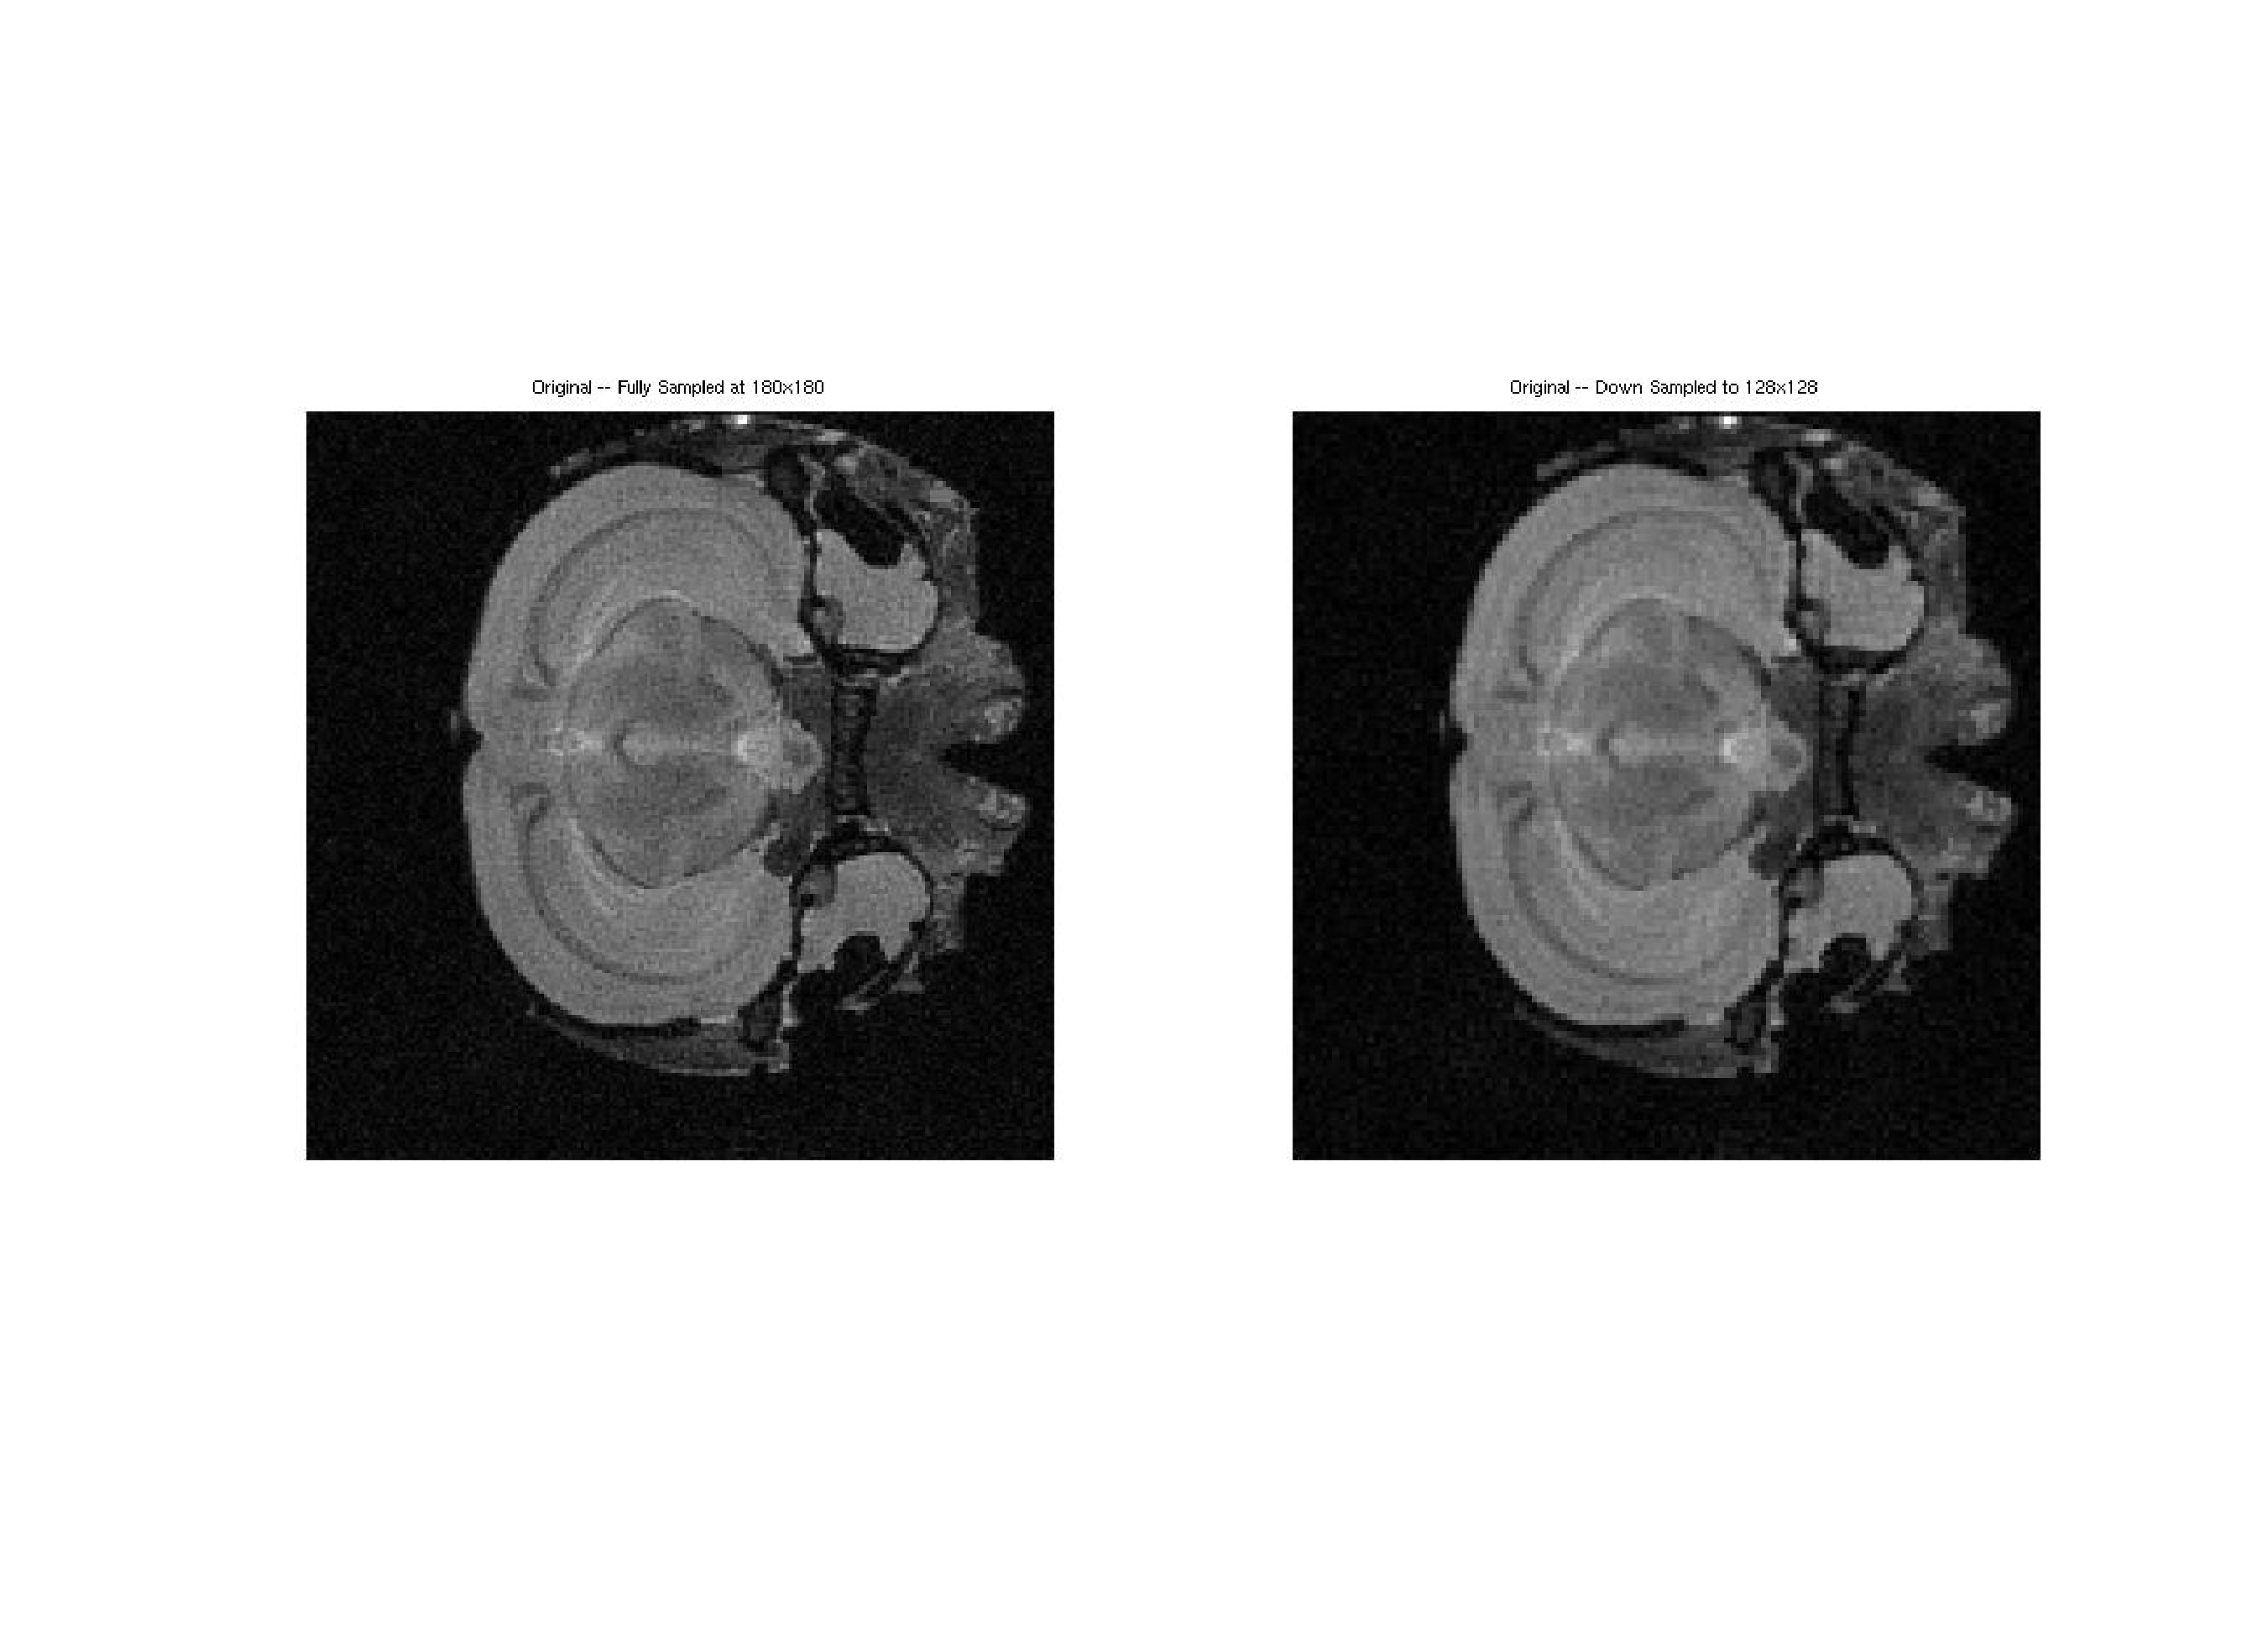
\includegraphics[trim = {60mm 100mm 46mm 70mm},clip,scale = 0.4] {Figs/CS_DTI_Sims/FullvsDownSample.eps}
    \caption{We can see the significant blurring effect that downsampling the figure to be 128x128 has. The blurring cannot be fixed, as in order to do this, we must sacrifice some higher spatial frequency information. Note that this is using \matlab blurring. This is explained further in the next section and figure 2.}
    \label{fig:dwnsamp}

  \end{figure}

  The downsampling is absolutely required because of how the wavelet transform is done. The 2D Wavelet transform has a $2^n$ size requirement in order to work (Lustig 2007, Yang 2015). We don't particularly care about the number of slices being $2^n$ as this will be fully sampled anyway. 

  It seems like \matlab does something a little weird with how it downsamples the FFT... It produces what looks like just a blurred copy of the image (as seen above) but it doesn't seem to get the data from the center, but instbuildLambdaead chooses the data in the top right section (before shifting) preferentially. This can be seen in Figure 2.

  \newpage
  \begin{figure}[h] 

    \centering
    \vspace{0pt}
    \setlength\fboxsep{0pt}
    \setlength\fboxrule{0.5pt}
    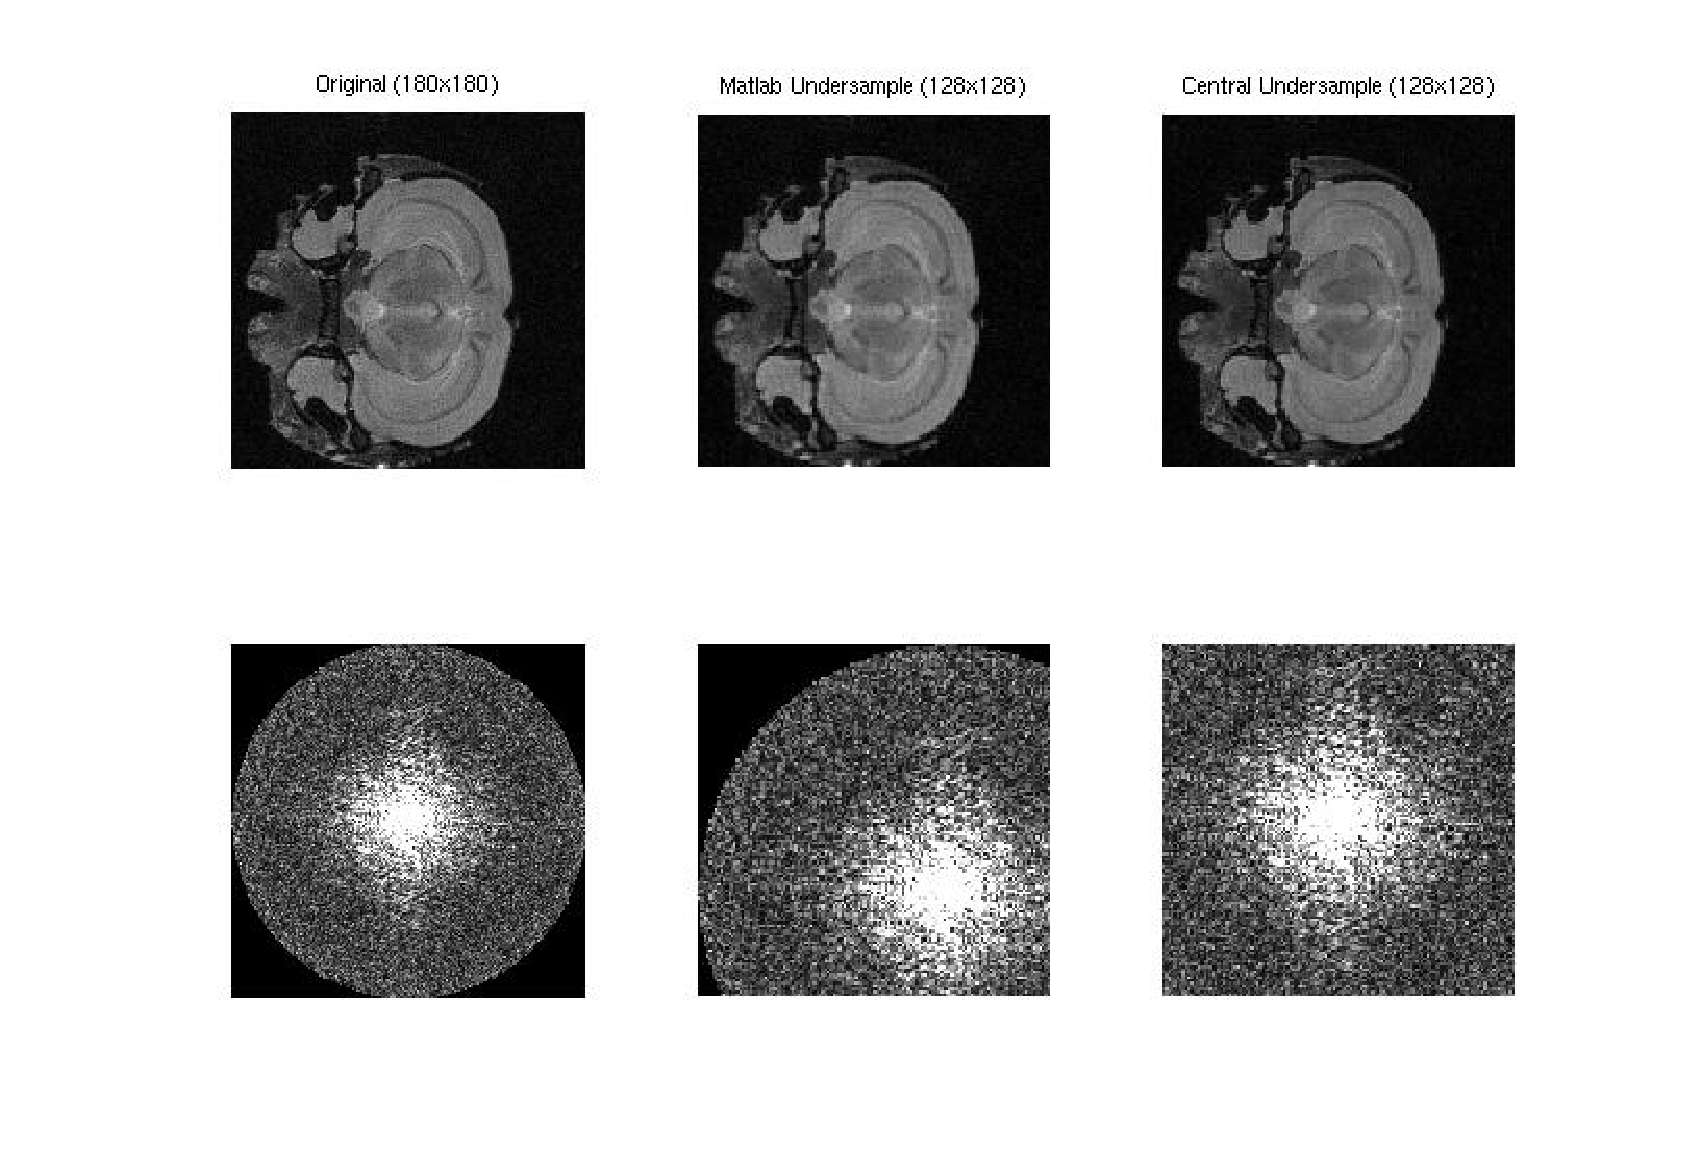
\includegraphics[trim = {36mm 20mm 20mm 8mm},clip,scale = 0.6] {Figs/CS_DTI_Sims/FullvsMatvsCent.eps}
    \caption{In this figure, we see some small differences between the method of undersampling done in \matlab vs a logical undersampling method that takes the data from the center of $k$-space. All data here taken from slice 150 \emph{after} doing a 1D FFT in the readout direction.}
    \label{fig:matvscent}

  \end{figure}

  We can see in the above figure that \matlab does something really weird and so, we will be using my method in order to do reconstructions that alter the number of voxels per dimension.

  In order to make sure that we're using the right one, the file we must use is \verb!kspaceDS.10.32.mat!, as this is the dataset that has been undersampled properly. For this work, what we will do right now, is look at how we can try to do a reconstruction properly using compressed sensing. We may be able to do this logically using some of the existing work here. In the angiography case, they use the previous slice as the base image as "not much is expected to change". We can do better than this, as we can try to do a combined reconstruction, where the $b_0$ average of the same slice (to start) would be the same. 

\section{Simulations - (03.11.15)}
\noindent 03.23.15 (work completed on and before 03.19.15)
  \subsection{Preamble}

  The point of running this simulation is to see what the best undersampling method to use would be. Our plan of attack is to do this experiment two fold, firstly with purely numerical data -- i.e. a ``phantom" that I design, and then afterwards using true brain data and seeing if we can get an understanding of what the best method would be. 
  
  Some of this information is noted at an earlier point in time, 

  \subsection{Hypothesis}

  The expectation is that the best style would be to use the ``parallel to the gradient direction" as this will give us the sharpest edge information in order to tell a cross section of the fibres that we are expecting to see. The worst should be the ``perpendicular" case. It is noted that our nomenclature from before was misleading. In order to ensure that we have it correctly, the following figure explains what is meant by each.

  % Directionality! figure
    \begin{figure}[h] 

    \centering
    \vspace{0pt}
    \setlength\fboxsep{0pt}
    \setlength\fboxrule{0.5pt}
    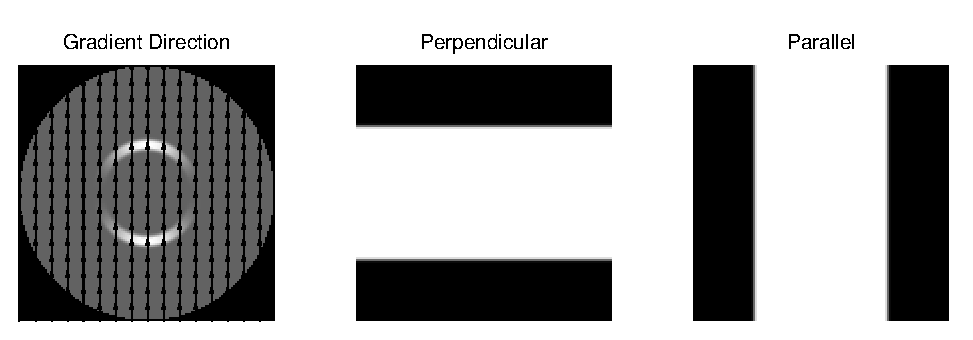
\includegraphics[trim = {0mm 0mm 0mm 0mm},clip,scale = 0.8] {Figs/numericalSims/GradDir01.eps}
    \caption{We can see the direction of the gradient in the left-most panel, and the definitions of the others. The parallel will give us the ``cross-fibre" information mostly, and the perpendicular will give us the ``along the fibre" information.}
    \label{fig:GradDir}

  \end{figure}

  \subsection{Results}
  
    \subsubsection{Numerical Simulations}
    
    For the numerical simulations, we started with a phantom that was comprised of three parts. The phantom can be seen in the following image.
    
    \begin{figure}[!h] 

      \centering
      \vspace{0pt}
      \setlength\fboxsep{0pt}
      \setlength\fboxrule{0.5pt}
      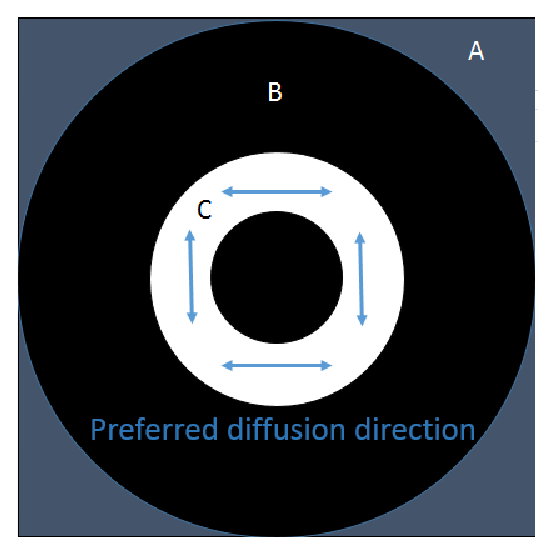
\includegraphics[trim = {0mm 0mm 0mm 0mm},clip,scale = 0.8] {Figs/numericalSims/Phantom.eps}
      \caption{This figure is the numerical phantom that we used. Region (A) represents an area of all zero data, used to serve as a reference point when plotting the figure (it forces the dynamic range to begin at zero). Region (B) represents an area of isotropic diffusion, where $\lambda_1 = \lambda_2 = \lambda_3 = 10^{-3}$. This area should have an FA value of zero. Region (C) represents an area with restricted diffusion, where $\lambda_1 = 10^{-3}$, but $\lambda_2 = \lambda_3 = 5 \times 10^{-4}$. This gives a theoretical FA value of approx $0.41$. It is noted that the $b$ value used in this experiment was 1917 $\frac{\text{s}}{\text{mm}^2}$}
      \label{fig:NumPhant}

  \end{figure}
    
    
    When we worked with this data, we used multiple different types of undersampling filters, and compared them to the fully sampled case. The ones that we used are:
    \begin{itemize}
      \item Circle
      \item Square
      \item Parallel Strip
      \item Perpendicular Strip
      \item Parallel Ellipse
      \item Perpendicular Ellipse
    \end{itemize}

    For the two ellipses, it is noted that the long axis to short axis ratio was set to be 2 (i.e. a/b = 2 if $\left(\frac{x}{a}\right)^2 + \left(\frac{y}{b}\right)^2 = 1$). It is also noted that $x$ and $y$ here are those of the axis rotated relative the gradient vector direction.
    
    % Talk about this more.
    Upon comparing all of our datasets, we found that the square and the circle gave the smallest RMS error. This can be seen via a bar chart -- this chart combined all the ROIs from all directions (doing the fully sampled - undersampled), and and ran an RMS on all of the data.
    
    \begin{figure}
      \centering
      \vspace{0pt}
      \setlength\fboxsep{0pt}
      \setlength\fboxrule{0.5pt}
      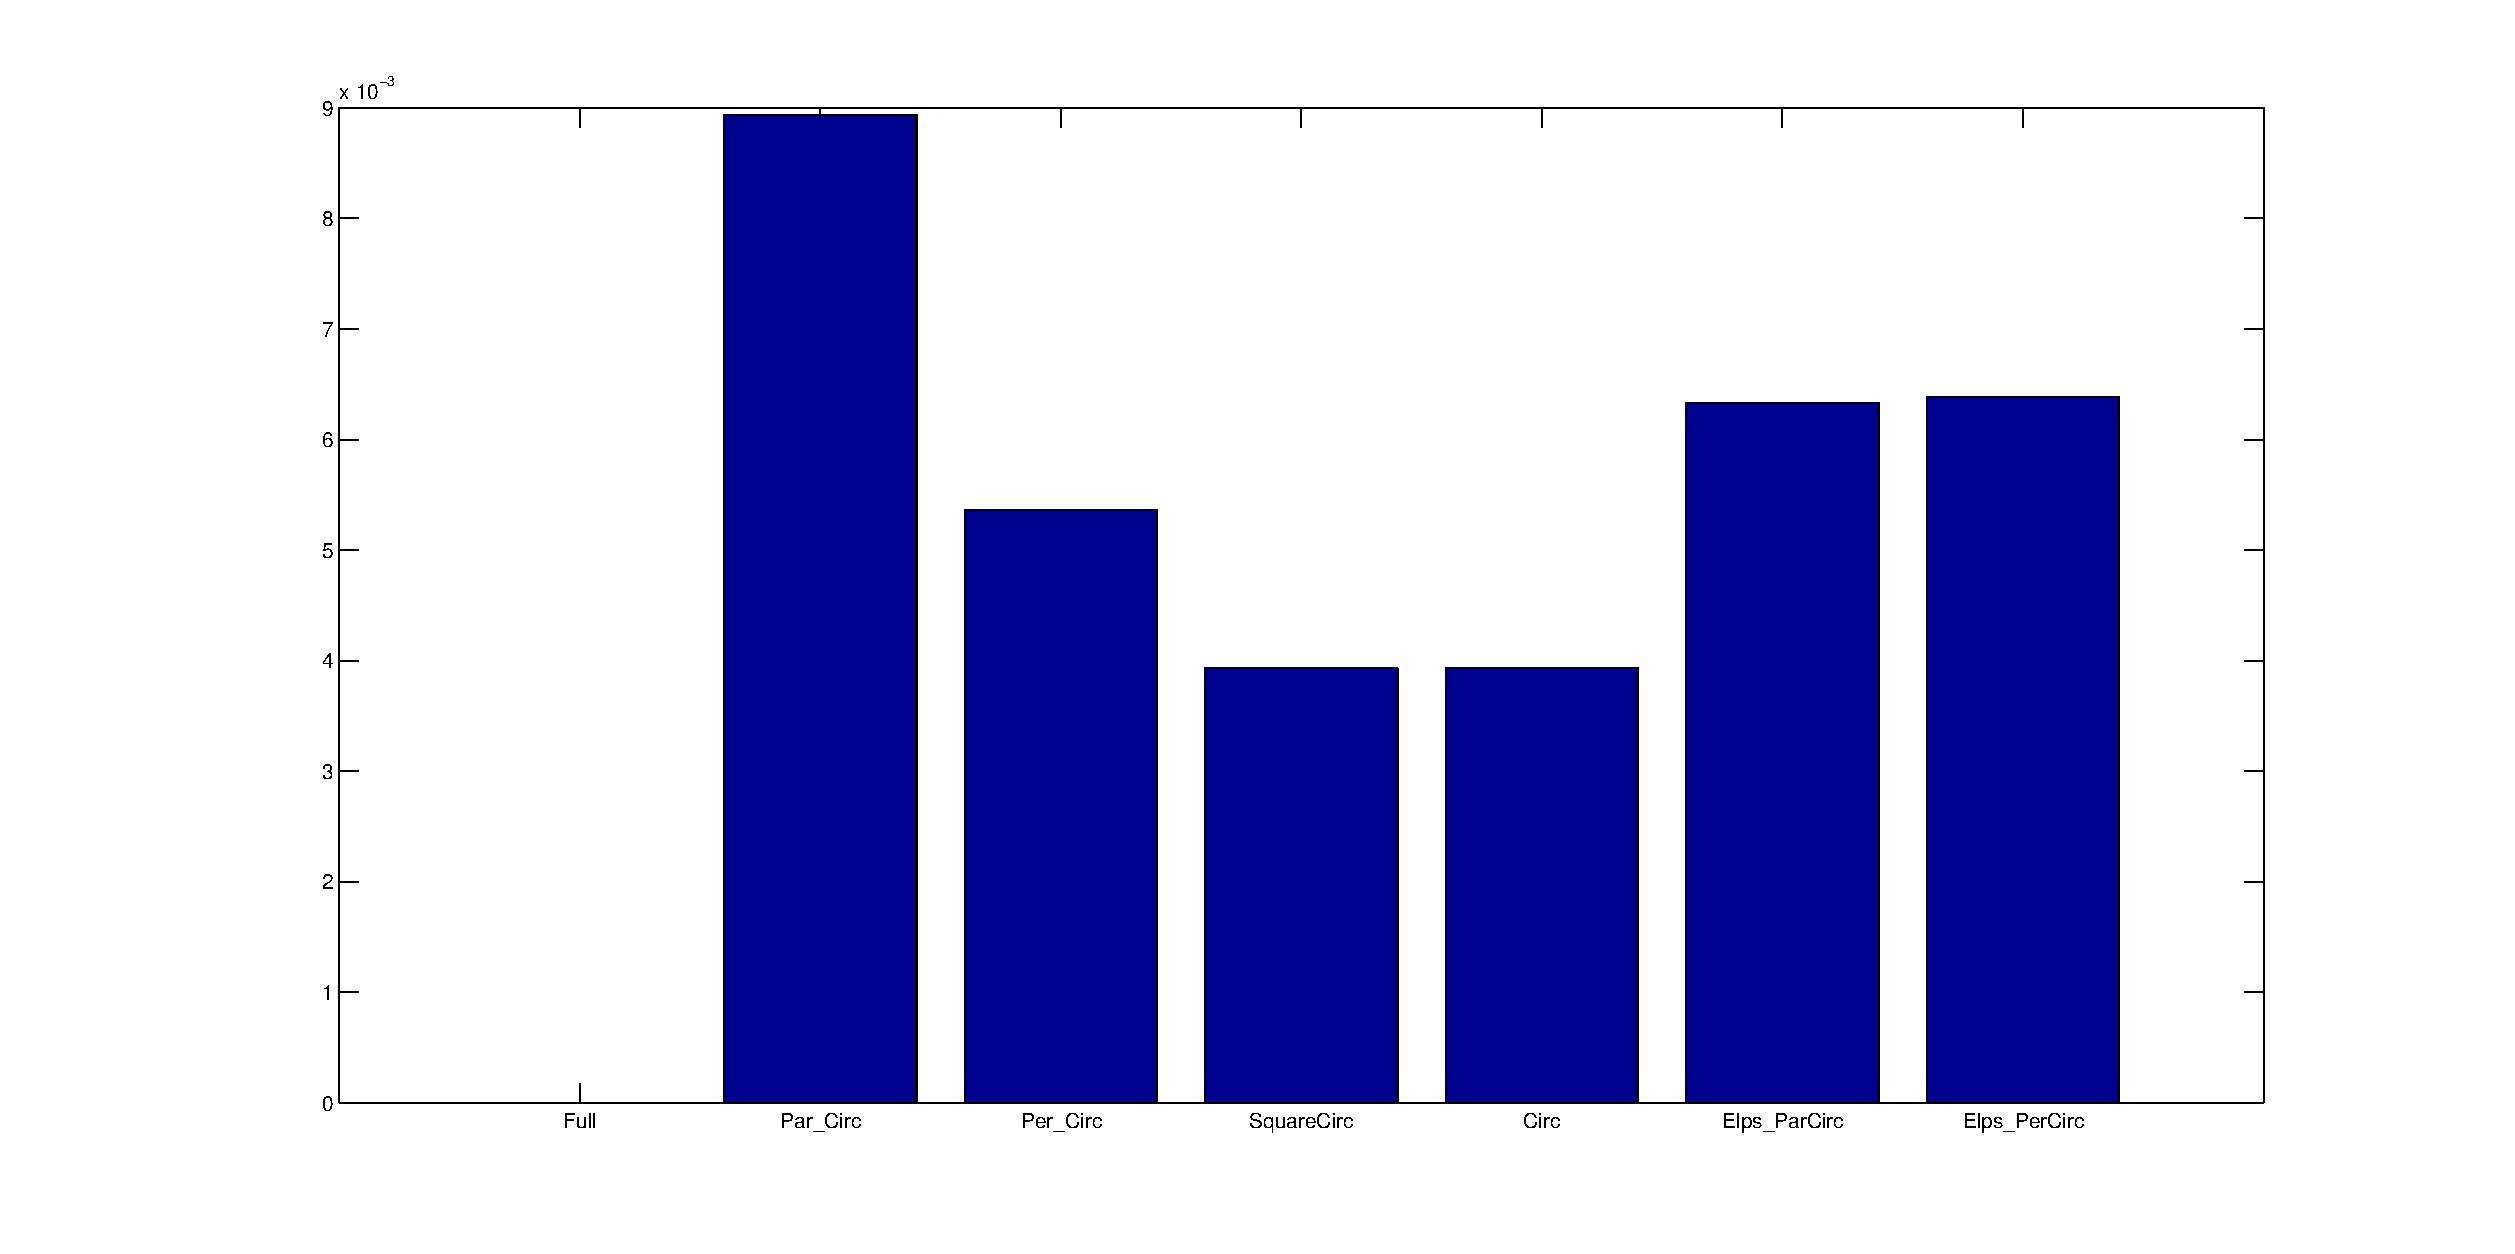
\includegraphics[trim = {10mm 0mm 10mm 0mm},clip,scale = 0.4] {Figs/numericalSims/nSimRMS.eps}
      \caption{This figure shows us how the RMS differs for the different undersampling types. We can see the undersampling types in the next figure.}
      \label{fig:RMSPhant}

  \end{figure}
  
  \begin{figure}
      \centering
      \vspace{0pt}
      \setlength\fboxsep{0pt}
      \setlength\fboxrule{0.5pt}
      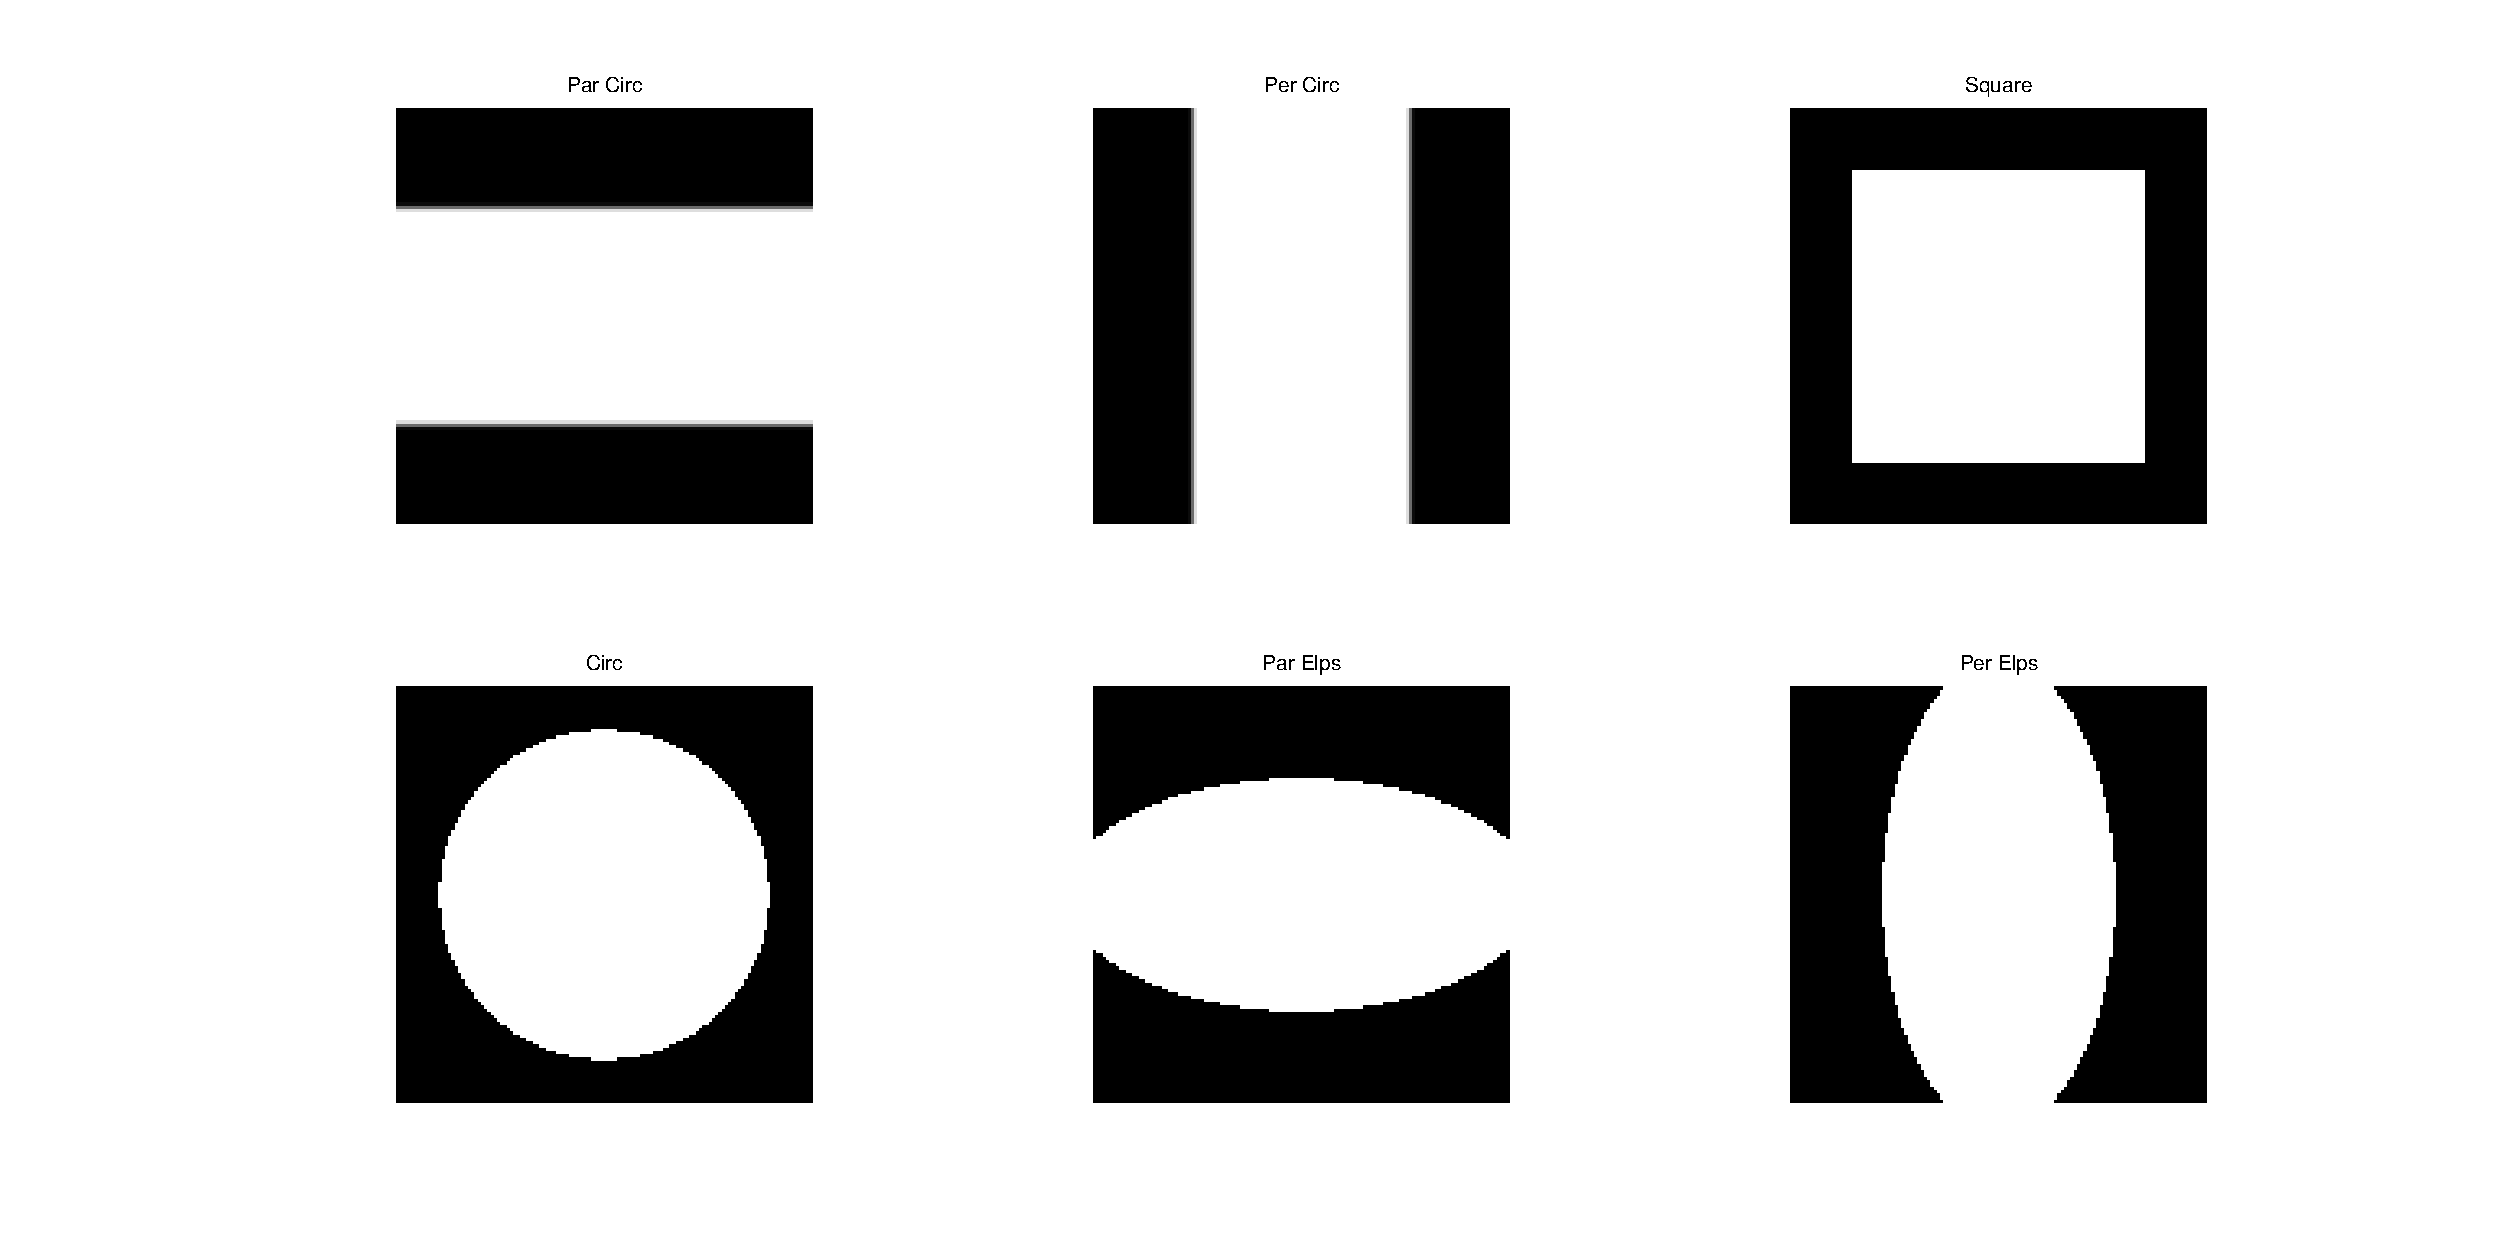
\includegraphics[trim = {10mm 0mm 10mm 0mm},clip,scale = 0.4] {Figs/numericalSims/DiffFilts.eps}
      \caption{The different filters that we used for the plots. It is noted that the codes used almost no roll off.}
      \label{fig:RMSPhant}

  \end{figure}
  
    \subsubsection{Brain Data}
    
    
  
  \subsection{Discussion}
  
  Surprisingly, we didn't particularly get what we expected. When running the simulation for the numerical phantom, the data didn't seem very different at all -- at least when comparing FA values. The data actually gave us results that were confounding... When being compared to the ``standard" methods of undersampling (i.e. Circular or low resolution undersampling), the parallel and perpendicular cases fell through and were not effective. However, we may be able to find some ``happy medium", as there may be an elliptical technique that has the lower RMS error of the circular technique, but the specificity of the directionally specific techniques.
  
  

\end{document}